%%%%%%%%%%%%%%%%%%%%%%%%%%%%%%%%%%%%%%%%%%%%%%%%%%%%%%%%%%%%%%%%%%%%%%%%%%%%
% AGUJournalTemplate.tex: this template file is for articles formatted with LaTeX
%
% This file includes commands and instructions
% given in the order necessary to produce a final output that will
% satisfy AGU requirements, including customized APA reference formatting.
%
% You may copy this file and give it your
% article name, and enter your text.
%
% guidelines and troubleshooting are here:

%% To submit your paper:
\documentclass[draft]{agujournal2019}
\usepackage{url} %this package should fix any errors with URLs in refs.
\usepackage{lineno}
\usepackage{placeins}
\usepackage{amsmath}

\usepackage[inline]{trackchanges} %for better track changes. finalnew option will compile document with changes incorporated.
\usepackage{soul}
\linenumbers
%%%%%%%
% As of 2018 we recommend use of the TrackChanges package to mark revisions.
% The trackchanges package adds five new LaTeX commands:
%
%  \note[editor]{The note}
%  \annote[editor]{Text to annotate}{The note}
%  \add[editor]{Text to add}
%  \remove[editor]{Text to remove}
%  \change[editor]{Text to remove}{Text to add}
%
% complete documentation is here: http://trackchanges.sourceforge.net/
%%%%%%%

\draftfalse

\newcommand{\aref}[1]{\textbf{Reference #1}}
\newcommand{\TODO}[1]{\textbf{TODO: \color{red}#1}}
\newcommand{\ian}[1]{{\textbf{\color{blue}Ian says:} \color{blue} #1} }
\newcommand{\mauro}[1]{{\textbf{\color{green}Mauro says:} \color{green} #1} }
\newcommand{\alpine}{\textit{ALPINE}\,}
\newcommand{\icesheet}{\textit{ICESHEET}\,}
\newcommand{\m}{$\,\mathrm{m}$\,}
\newcommand{\cm}{$\,\mathrm{cm}$\,}
\newcommand{\mma}{$\,\mathrm{mm  \, a^{-1}}$\,}
\newcommand{\mmma}{$\,\mathrm{m^3\, a^{-1}}$\,}
\newcommand{\mmms}{$\,\mathrm{m^3\, s^{-1}}$\,}
\newcommand{\unit}[1]{$\mathrm{#1}$}


\journalname{Geophysical Research Letters}


\begin{document}


\title{Water discharge quantity has a variable impact on sediment transport capacity in subglacial channels}


\authors{Ian Delaney\affil{1},  Andrew J. Tedstone\affil{2},   Mauro A. Werder\affil{3,4},  Daniel Farinotti\affil{3,4}, }

\affiliation{1}{Institut des dynamiques de la surface terrestre (IDYST), Universit\'{e} de Lausanne, B\^{a}timent G\'{e}opolis, 1015 Lausanne, Switzerland}
\affiliation{2}{Department of Geosciences, University of Fribourg, Ch. du Musée 1700, Fribourg, Switzerland}
\affiliation{3}{Laboratory of Hydraulics, Hydrology and Glaciology (VAW), ETH-Z\"urich, H\"onggerbergring 26, 8093 89 Z\"urich, Switzerland}
\affiliation{4}{Swiss Federal Institute for Forest, Snow and Landscape Research (WSL) Z\"uricherstrasse 111, 8903 1011 Birmensdorf, Switzerland}


\correspondingauthor{Ian Delaney}{ianarburua.delaney@unil.ch}

\begin{keypoints}
\item Water discharge variations in subglacial channels are mainly accommodated by water velocity, not channel size.
\item Greater variability in water velocity causes sediment transport capacity to vary more in subglacial channels than in subaerial channels.
\item Water discharge may represent processes including proglacial sediment mobilization and sediment access driving variations in sediment discharge, as opposed to subglacial sediment transport capacity in glacierized catchments.
\end{keypoints}

\begin{abstract}
  Sediment transport capacity in subglacial and subaerial channels depends on  water velocity and channel width, which together control the shear stress exerted on the channel bottom.
  In subaerial channels, width, and velocity evolve quickly with water discharge, while in subglacial channels, water discharge changes mainly affect water velocity due to slow-evolving channel geometry.
  Parameterizations of these subglacial and subaerial hydraulics are applied to hydrographs from an Alpine glacier and the Greenland Ice Sheet revealing greater variability in sediment transport capacity in subglacial channels.
  Furthermore, results show that high subglacial sediment transport rates can persist across various water discharges.
  Slowly evolving channel width accommodates some variability in subglacial channels.
  Despite differences in response to water discharge, sediment discharge measurements generally correlate better with subaerial hydraulic parameters.
  This implies that other factors like sediment access or proglacial processes might be at play, affecting sediment transport capacity differently in subglacial and subaerial channels.
\end{abstract}

\section{Introduction}
\label{sect:intro}

Changes in glacier dynamics, geomorphology, and hydrology  have prompted numerous  recent studies of  sediment transport processes in cold regions \cite<e.g.>{zhang2022}.
Increases in sediment transport  have been observed in Greenland \cite{bendixen2017}, the European Alps \cite{costa2017}, the Himalayas \cite{li2021}, and the Andes \cite{vergara2022}.
In some regions, increased water discharge and glacier melt have been interpreted to yield greater sediment transport capacity \cite{bendixen2017,costa2017,li2021}.
Observed changes to sediment transport in glacierized catchments require examining the processes controlling sediment discharge in these catchments and its variations with water discharge  \cite<e.g.>{riihimaki2005,swift2005}.

Over long periods, processes such as glacier abrasion and quarrying sculpt landscapes and create sediment to be transported fluvially from under glaciers \cite<c.f.>{hallet1979,iverson2012,ugelvig2018}.
On shorter time periods, pressurized water transports sediment from underneath glaciers \cite{walder1994,creyts2013,beaud2018,delaney2019}, should enough sediment be present subglacially (i.e. in a transport-limited regime).

In a transport-limited regime, sediment discharge responds to the sediment transport capacity, defined as the amount of sediment the water can carry.
Sediment transport capacity depends on the shear stress between water and the sediment it flows  over \cite{shields1936,meyer1948,engelund1967} along with the width of the channel bottom $w_c$ over which to mobilize sediment.
The shear stress  across the channel width $\tau_t$ responds to the velocity of water $v$ flowing through the channel so that
\begin{linenomath*}
  \begin{equation}
    \label{eq:tau_t}
    \tau_t \propto w_c\, v^2,
  \end{equation}
\end{linenomath*}
%
where $w_c$ is the width of the channel. Following mass conservation, the velocity of the water flowing through a  channel is
\begin{linenomath*}
  \begin{equation}
    \label{eq:v}
    v = \frac{Q}{S},
  \end{equation}
\end{linenomath*}
where $Q$ is water discharge,  and $S$ is the channel's wetted area.

In subaerial channels, operating with open channel flow, the wetted area $S$ of the channel evolves with changing water discharge $Q$, by changing both the channel's width and the water depth \cite{leopold1953}.  The change in water depth results in a commensurate increase in water velocity.  Thus,  fulfilling Equation~\ref {eq:v}, the higher discharge is accommodated by both an increase in wetted area and flow velocity. As a result, the shear stress across the channel $\tau_t$ increases according to Equation~\ref{eq:tau_t}.

The response of water velocity to changing water discharge in subglacial channels differs from subaerial ones.
The size of subglacial channels responds to the creep closure of the ice above and the opening of the channel by frictional heating of water flowing through the channel \cite{rothlisberger1972}.
As a result, the subglacial channel size only evolves relatively slowly over days to months, whereas water discharge can vary over hours \cite<e.g.>{iken1986,andrews2014,nanni2020}.
Therefore, subglacial water flow behaves more like pipe flow, and changes in water discharge $Q$ are mainly accommodated with increased or decreased water velocity $v$ \cite{alley1997} because the size of the channel $S$ changes on a much longer timescale (Equation~\ref{eq:v} and Figure~\ref{fig:cartoon}).
It follows that an increase in water discharge $Q$ will cause the shear stress across the channel $\tau_t$ to respond with water velocity $v$, as opposed to subaerial channels where channel width $w_c$ evolves as well.

  \begin{figure}[h]
  \centering
    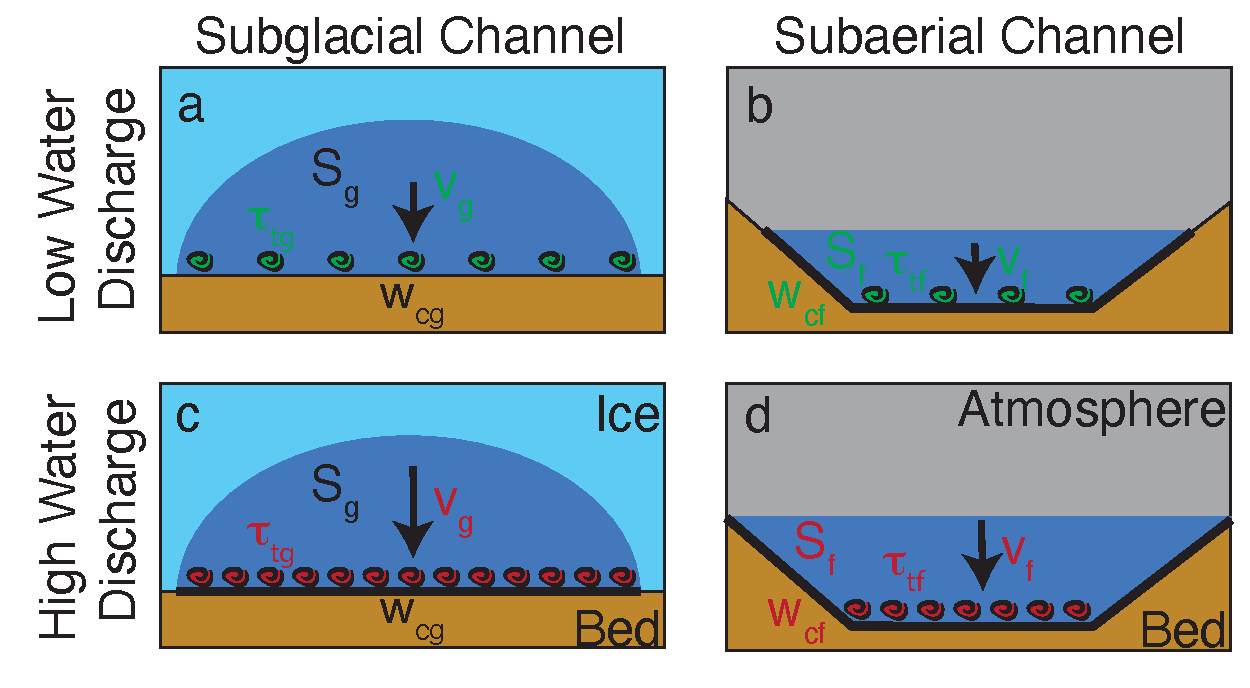
\includegraphics[width=0.8\linewidth]{Fig1.pdf}
    \caption{Sketch for the different responses that subglacial and subaerial channels have to an increase in water discharge.  Water velocity magnitudes in the subglacial, $v_g$, and subaerial, $v_f$, channels are shown by arrow length. $S_g$ and $S_f$ represent the wetted area in subglacial and subaerial channels, respectively. The subglacial channel widths $w_{cg}$ remain unchanged, while the subaerial channel widths $w_{cf}$ evolve. Shear stress $\tau$ is responsible for the mobilization of sediment and increases with the number of makers at the channel bed.
      Note that in the subaerial channel parameterization, channels have rectangular shapes with their width much larger than their depth (Section~\ref{sect:fluv}).}
    \label{fig:cartoon}
  \end{figure}
% \ian{Come back to Daniel's comments}

As a result, sediment mobilization in subaerial and subglacial channels responds differently to changing water discharge.
These differences have been implicitly included in a wide range of available models that  quantify sediment transport from catchments in both subglacial and subaerial channels  \cite<e.g.>{walder1994,alley1997,tucker1997,creyts2013,delaney2019,hewitt2019,wickert2019}.
The divergent response of changing water discharge on sediment mobilization capacity may well impact sediment dynamics at glacier margins where flow transitions from pressurized to open channel flow \cite<e.g.>{lane2016,perolo2018}.
Additionally, the variable response of sediment transport capacity to water discharge in the two systems may affect the interpretation of sediment transport records in glacial systems \cite<e.g.>{muller1968,richards2003,swift2005,ganti2016}.
Yet, little work has examined the differing relationship between variations in water discharge and sediment discharge in subglacial and subaerial channels \cite{alley1997}.
%Furthermore, thorough observations of water velocity and channel width in subglacial channels are limited and, to these authors' knowledge, not contrasted with subaerial conditions at the glacier margins. %\mauro{self-cite here?}

This manuscript evaluates the relationship between sediment transport capacity and water discharge in subglacial channels, and compares it to subaerial ones.
In the absence of continuous measurements of subglacial and subaerial water velocity and channel morphology, numerical parameterizations of subglacial and subaerial hydraulics are utilized.
Parameterizations are applied to hydrological records from an Alpine glacier in Switzerland (Fieschergletscher) and  a land-terminating glacier in Greenland (Leverett Glacier).
The parameterizations' lumped nature isolates the disparity between water discharge and sediment transport capacity in subglacial systems, independent of the upstream drainage network and sediment access.
Outputs demonstrate differences in the relationships between  water discharge, channel geometry, and water velocity in the subglacial and subaerial channels.
Furthermore, outputs are compared to sediment discharge data from these two catchments.
The manuscript then uses the demonstrated differences between the two channel types to discuss the implications for interpreting the processes driving variability in records of sediment transport from glacierized catchments.

\section{Study sites and data}
\label{sect:ss_data}

Water and suspended sediment data are leveraged from Alpine and ice sheet settings.
The Alpine site (\alpine) is  Fieschergletscher in the Swiss Alps ($46^\circ\,29'\,07''$ N, $8^\circ\,08'\,3''$ E).
Water discharge and suspended sediment concentration were collected here at a $1$\unit{min} interval continuously over the period 2014--2021.
See \citeA{felix2022} and \citeA{felix2021} for more details.

The Leverett Glacier in Greenland (\icesheet) serves as the ice sheet setting.
Water discharge and suspended sediment concentration data were collected roughly $2$\unit{km} downstream from the terminus between June and August/September 2009 to 2012 ($67^\circ\,03'\,5''$ N, $50^\circ\,12'\,59''$ W).
Data is used from \citeA{tedstone2017} and \citeA{hawkings2014} at a $5$\,\unit{min} time interval from May 28, 2012 to August 8, 2012.
Two gaps in suspended sediment data of roughly one day in length are interpolated across with a linear spline.

\section{Methods}
\label{sect:meth}
The parameterizations below (Sections ~\ref{sect:sub_mode}~and~\ref{sect:fluv}) represent relationships amongst water discharge, water velocity, and channel geometry in both subaerial and subglacial channels (Table \ref{table:vpm}).
Both parameterizations calculate   water velocity, shear stress, and width-integrated shear stress, upon which sediment transport depends \cite<Figure \ref{fig:cartoon}; >{shields1936}.
The evaluation of these variables omits the selection of a sediment transport relationship and a grain-size parameter \cite<e.g.>{shields1936,meyer1948} needed to calculate sediment transport capacity from shear stress.


\subsection{Subglacial channel  parameterization}
\label{sect:sub_mode}

To evaluate the shear stress of water flowing across sediments underneath a glacier, the subglacial channel parameterization takes into account the channel geometry and the velocity of the flowing water.
To do this, a modified version of the lumped hydraulics model presented in \citeA{clarke1996} and \citeA{werder2010} is used.

Here, it is assumed that the water is transported through a subglacial channel \cite<Figure~\ref{fig:cartoon}; >{rothlisberger1972}, and that the channel  size responds to frictional heating from water flow and creep closure by ice, using the Darcy-Weisbach formulation for water-flow through a pipe  \cite<e.g.>{rothlisberger1972,clarke2003}.
The formulation here does not consider the englacial storage of water.
Thus, it is assumed that the changing hydraulic head at the top of the glacier is negligible in the channel size evolution.
The evolution of subglacial channel size $S_g$ is given as
\begin{linenomath*}
  \begin{equation}
    \label{eq:dS_dt}
    \frac{\partial S_g}{\partial t} = C_1 \frac{Q \Delta h}{l} - C_2 \left(h_{o}-\frac{\Delta h}{2}\right)^n\,S_g,
  \end{equation}
\end{linenomath*}
\noindent where $C_1= (1-\rho_wc_pc_t)\,\frac{\rho_wg}{\rho_iL}$ and $C_2=2A(\frac{\rho_wg}{n})^n$ are constants (Table \ref{table:vpm}), $l$ is the length of the subglacial channel, $Q$ is water discharge, $\Delta h$ is the hydraulic potential change from the glacier terminus to its top, $h_{o}= \frac{\rho_i}{\rho_w} h_{ice}$ is the ice overburden pressure, and $n$ is Glen's n \cite{glen1955} (usually $n=3$).
The first term on the right side of the equation represents the opening of the channel through frictional heating, while the following term represents the creep closure of the channel from ice deformation.


Following the Darcy-Weisbach equation, head drop $\Delta h$ is,
\begin{linenomath*}
  \begin{equation}
    \label{eq:dh}
    \Delta h \,  = l \,\frac{1}{g}\,s\,f_r\,\frac{Q^2}{D_h^5}
  \end{equation}
\end{linenomath*}
\noindent where $f_r$ is a friction factor, $D_h$ is the hydraulic diameter, and $l$ is the length over which head change occurs. $s$ is a factor accounting for channel geometry \cite{hooke1990}, calculated as
\begin{equation}
  \label{eq:Hf}
  s = \frac{2\,(\beta -\sin \beta)^2}{(\frac{\beta}{2}\,+\,\sin \frac{\beta}{2})^4},
\end{equation}
where $\beta$ is the central angle of the circular segment that comprises the channel (the so-called Hooke angle). Note that $\beta =\pi$ corresponds to a semi-circle and
smaller values of $\beta$ result in shallow, wide channels.
The hydraulic diameter $D_h$ is converted to wetted area $S_g$ given a channel geometry following \cite{hooke1990}
\begin{equation}
  \label{eq:Dh2S}
  S_g= \frac{D_h^2}{2}\,\frac{(\frac{\beta}{2}+\sin \frac{\beta}{2})^2}{\beta - \sin \beta}.
\end{equation}


With knowledge of wetted area $S_g$, the shear stress, $\tau_g$, between the water and the channel bed is determined through the Darcy-Weisbach formulation
\begin{equation}
  \label{eq:tau}
  \tau_g=\frac{1}{8}\,f_r\,\rho_w\,v_g^2,
\end{equation}
%
where $v_g = \frac{Q}{S_g}$ is the water velocity.

The width-integrated shear stress is represented as
\begin{equation}
  \label{eq:tautg}
  \tau_{tg}=w_{cg}\,\tau_g,
\end{equation}

where $w_{cg}$ is the flat channel floor width:
\begin{equation}
  \label{eq:dh2wc}
  w_{cg} = 2  \sin \frac{\beta}{2} \sqrt{\frac{2\, S_g}{\beta -\sin \beta}}.
\end{equation}

\subsection{Subaerial channel  parameterization}
\label{sect:fluv}

To parameterize the shear stress of water flowing across sediments in the subaerial channel,  the hydraulics parameterization presented in \citeA{tucker1997} is implemented.
Using mass conservation and the Darcy-Weisbach relationship as well as assuming that the channel is wide so that the hydraulic radius is well approximated by the flow depth, then
the shear stress $\tau_f$ at the river bed is
\begin{linenomath*}
  \begin{equation}
    \label{eq:DW_tau}
    \tau_f=\frac{\rho_w\,g^{\frac{2}{3}}\,f_p^{\frac{1}{3}}}{2}\, \Big(\frac{Q}{w_{cf}} \Big)^{\frac{2}{3}} \,\nabla z_c^{\frac{2}{3}},
  \end{equation}
\end{linenomath*}
where $\nabla z_c$ is the channel slope, and $f_p$ is the friction factor for subaerial channels.
Channel width $w_{cf}$ is
\begin{equation}
  \label{eq:wcf}
  w_{cf} = k \, Q^\frac{1}{2},
\end{equation}
%
where $k$ is a constant and $\frac{1}{2}$ is a commonly chosen exponent \cite{leopold1953}.
%\mauro{This is for so called ``regime channels''}
Water velocity, $v_f$, is given by rearranging Equation \ref{eq:tau} as
\begin{equation}
  \label{eq:vf}
  v_f = \sqrt{\frac{8\,\tau_f}{f_p\,\rho_w}}.
\end{equation}
%
As above, the width-integrated shear stress is
\begin{equation}
    \label{eq:tautf}
    \tau_{tf}=w_{cf}\,\tau_f.
  \end{equation}

\subsection{Implementation}
\label{sect:imp}

The parameterizations above are applied to hydrological records from the Fieschergletscher (\alpine) and the Leverett Glacier (\icesheet).
The subglacial and subaerial parameterizations represent the subglacial flow of water exiting a glacier and transitioning to subaerial flow, as it moves through the catchment.
Outputs of the parameterizations are meant to represent generalizable sediment transport characteristics from these hydrographs, rather than actual hydraulic conditions.
To generalize these cases, \alpine{}  is exemplified by relatively thin ice thickness ($h_{ice}$: $225$\,\unit{m}), low water discharge ($\sim\,10$\,\unit{m}$^3$\,\unit{s}$^{-1}$) and high diurnal variability in water discharge (Figure~\ref{fig:model_outs}, a).
\icesheet{}  is exemplified by thick ice  ($h_{ice}$: $700$\,\unit{m}), high water discharge ($\sim\,300$\,\unit{m}$^3$\,\unit{s}$^{-1}$)  and low diurnal variability in water discharge (Figure~\ref{fig:model_outs}, e).

For each glacier, the parameterizations are first applied to a reference test case for each glacier that assumes  subglacial channel with $\beta=\frac{\pi}{2}$. Friction factors $f_r$ and $f_p$ are tuned so that the parameterizations reproduce reasonable water velocities for both \alpine and \icesheet{}\cite<$\sim\,1.6\,$\unit{m}$^3$\,\unit{s}$^{-1}$>{werder2010b,chandler2013}.
In both subaerial channels, the bed slope is $\nabla z_c = 0.05$.
Water velocity, shear stress, and width-integrated shear stress in the subglacial and subaerial channels from this formulation are presented below.

Second, to characterize the variability in sediment discharge capacity in subglacial compared to subaerial channels further, $100$  parameterizations are applied to a range of different channel geometry factors ($\beta$ and $k$) and friction factors ($f_r$ and $f_p$).
Runs with parameter combinations are culled if their mean subglacial water velocity over the season lies outside of the range between $0.75$\,\unit{m}$^3$\,\unit{s}$^{-1}$ and $2$\,\unit{m}$^3$\,\unit{s}$^{-1}$ or if subaerial water velocity lies outside of the range $0.3$\,\unit{m}$^3$\,\unit{s}$^{-1}$ and $1.2$\,\unit{m}$^3$\,\unit{s}$^{-1}$, in accordance with measurements \cite<e.g.>{werder2010b,magnusson2012,chandler2013}.
The standard deviation of an output over the course of the season is used to quantify its variability.

Lastly,  outputs are compared with the sediment discharge records of the glaciers using Spearman rank correlation, that is the correlation with respect to the ordering of values from the outputs and the observations.
Rank correlation reduces the impact of the non-linear response of sediment transport capacity to the hydrological forcing.
Outputs and observations, which have a native time resolution of $5$\,\unit{min}, are aggregated across timescales from $15$\,\unit{min} to $15$\,\unit{days} by averaging values one half of the timescale before and after a given point time.


\section{Results}

\subsection{Role of water discharge in sediment transport capacity}
\begin{figure}[h]
  \centering
  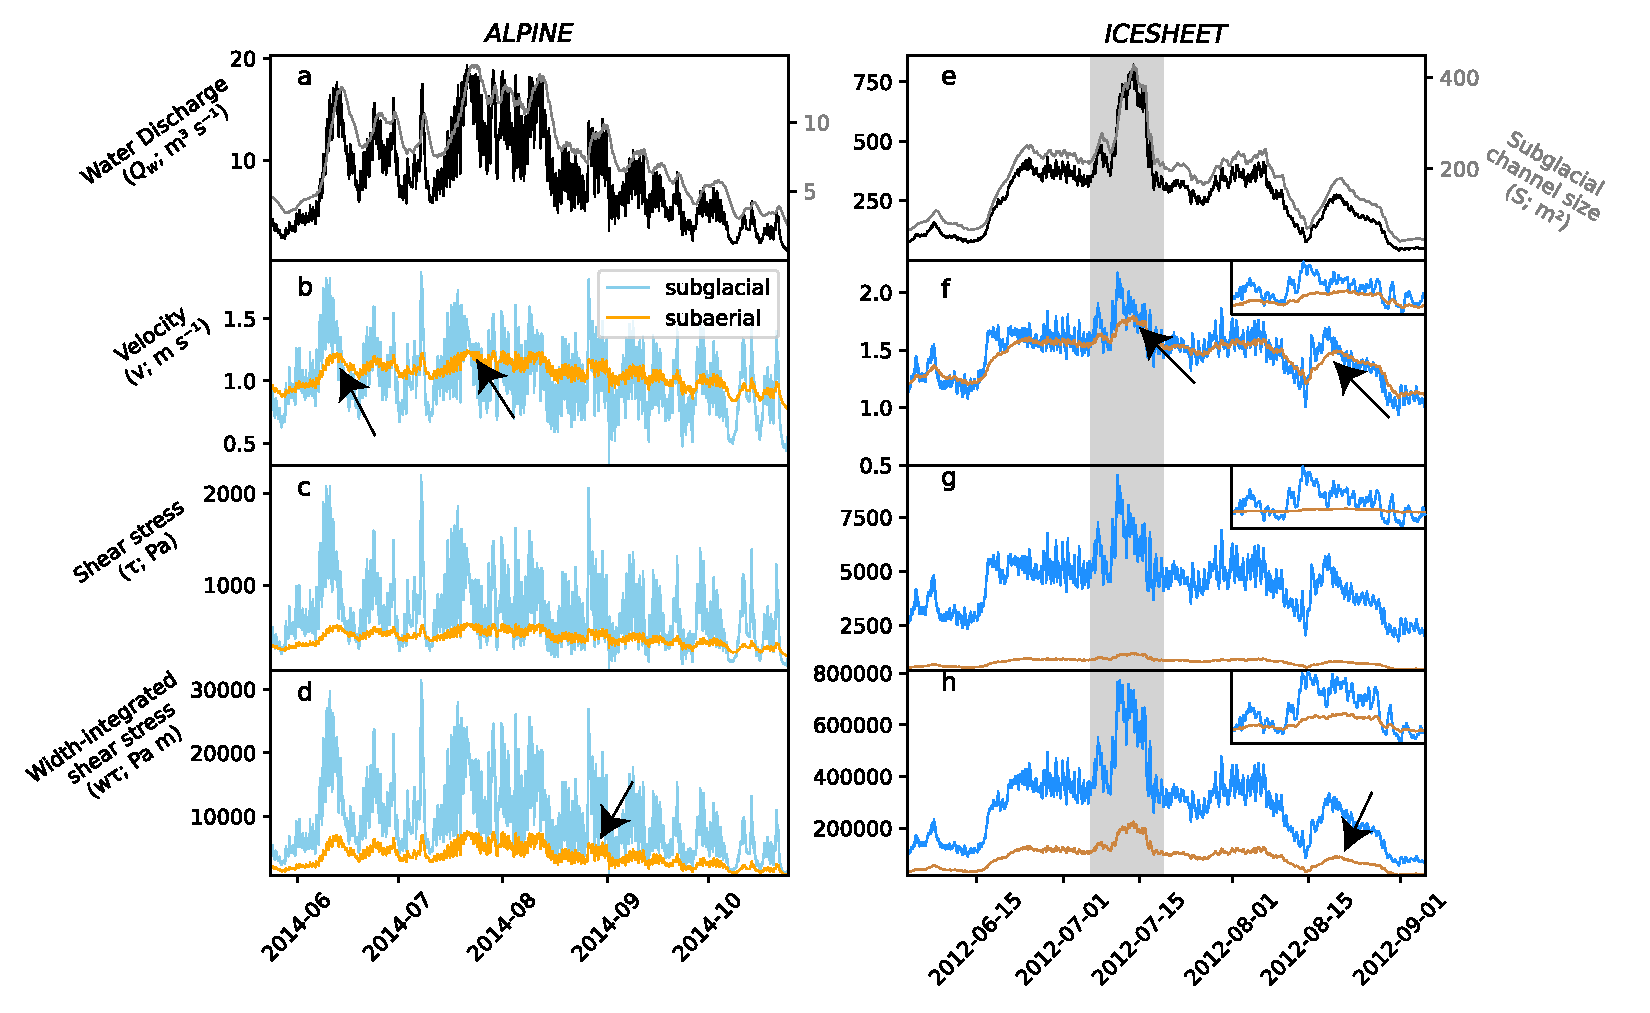
\includegraphics[width=0.9\linewidth]{Fig2.pdf}
  \caption{Parameterization outputs resulting from the hydrographs shown in panels a and e for the cases called \alpine (a-d) and \icesheet{} (e-h). Gray (black) lines in a and e represent the subglacial channel size (water discharge).  In other panels, blue lines represent outputs from the subglacial channel, while orange lines represent the subaerial channel.
    Data are shown at $15$\unit{min} intervals.
    Arrows denote some events where the variables peaks in the subglacial channel prior to the subaerial one.
    Insets in e-h show the  peak melt event \icesheet{} denoted by the shaded area.
    Note that the x and y axes are different for \alpine{} and \icesheet{}.
      }
  \label{fig:model_outs}
\end{figure}
Following the parameterizations defined in Sections~\ref{sect:sub_mode}~and~\ref{sect:fluv}, the water velocity, shear stress, and width-integrated shear stress exhibit different seasonal evolutions and peaks. Water velocity and shear stress represent the potential for sediment mobilization, and width-integrated shear stress represents a proxy for the total sediment transport capacity across the channel bed (Figure~\ref{fig:model_outs}).

Over the course of the season, large peaks in water velocity and shear stress, along with width-integrated shear stress, occur in response to increases in water discharge in both \alpine{} and \icesheet{}.
This occurs as the subglacial outputs are generally larger than the subaerial values, thus more efficient at transporting sediment.
In the subglacial channel, peaks generally occur over the period when water discharge increases at the fastest rate (Figure~\ref{fig:model_outs}).
Alternatively, in the subaerial channel, peaks in these sediment transport variables occur when water discharge is highest.
The timing of the greatest rate of change in water discharge occurs before the peaks in water discharge.
Here, sediment could be deposited in the proglacial area as the water depressurizes, then remobilized when sediment transport capacity peaks in the subaerial system.

\begin{figure}[h]
  \centering
  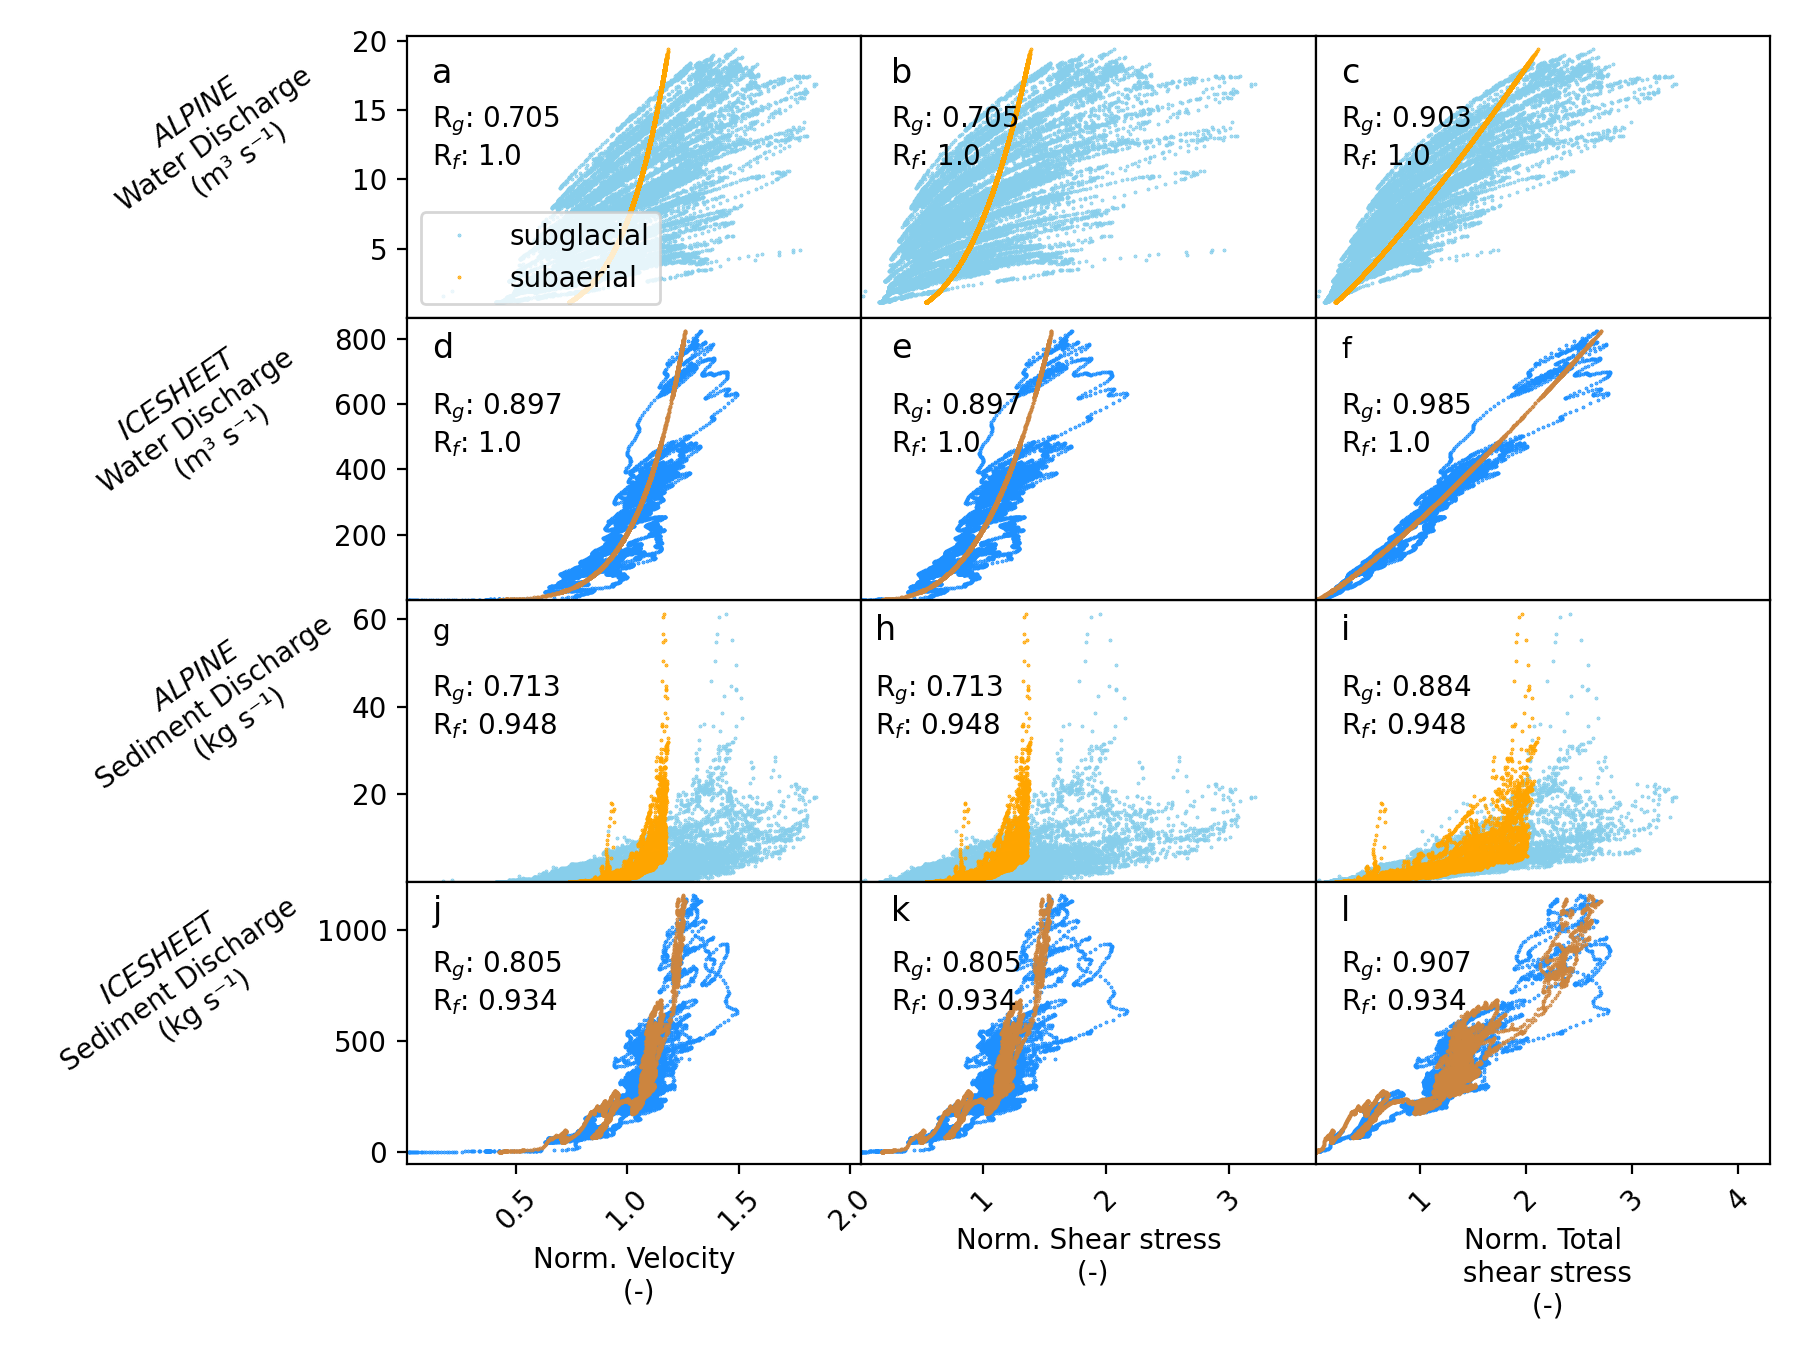
\includegraphics[width=0.9\linewidth]{Fig3.png}
  \caption{Relationship between water discharge and velocity, shear stress, and width-integrated shear stress for \alpine{} (a-c) and \icesheet (d-f).
    These outputs' relationship with measured sediment discharge is given for \alpine in (g-i) and \icesheet (j-l).
    Variables have been normalized to mean values for better comparison amongst the runs.
    $R_g$ and $R_f$ show the Spearman rank correlation values for the subglacial and the subaerial outputs, respectively.
    Plots are shown with data and outputs at $15$\unit{min} intervals.
  }
  \label{fig:Qw_vari}
\end{figure}

Each water discharge value in the subaerial channel results in a unique water velocity, shear stress, and width-integrated shear stress, creating a perfect rank correlation between the variables (Figure~\ref{fig:Qw_vari} a--f).
In the subglacial channel, however,  the outputs can vary substantially for a given water discharge and width-integrated shear stress varies with respect to the other two  outputs as well (Figure~\ref{fig:Qw_vari} a--f).
For instance, very high  water velocity values and shear stresses can occur across minimal water discharge at $2.5$\,\unit{m}$^3$\,\unit{s}$^{-1}$ to the maximum water discharge at over $17$ \,\unit{m}$^3$\,\unit{s}$^{-1}$.
In \icesheet, mean values of water velocity can occur at water discharges between roughly $150$ \,\unit{m}$^3$\,\unit{s}$^{-1}$ and $310$ \,\unit{m}$^3$\,\unit{s}$^{-1}$.

When considering the subglacial channel's evolving width, width-integrated shear stress  across the channel generally increases with water discharge, with improved rank correlation compared to water velocity or shear stress (Figure~\ref{fig:Qw_vari} a--f).
Yet even the width-integrated shear stress  can vary substantially, with the highest values occurring at water discharge values ranging from roughly $11$ \,\unit{m}$^3$\,\unit{s}$^{-1}$ to over $17$ \,\unit{m}$^3$\,\unit{s}$^{-1}$.
The variability in width-integrated shear stress is less pronounced in the \icesheet case, with reduced variability in water discharge (Figure~\ref{fig:Qw_vari} c, f).
The persistence of high water velocity, shear stress, and width-integrated shear stress suggests that substantial sediment transport may occur across much of the water discharge range in the subglacial system (Figure~\ref{fig:Qw_vari} a--f).


\begin{figure}[h]
  \centering
    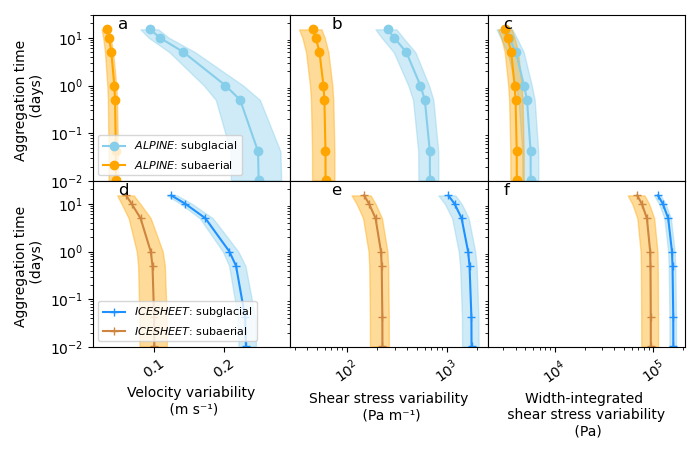
\includegraphics[width=0.9\linewidth]{Fig4.png}
    \caption{Variability (measured by the standard deviation) in water velocity, shear stress, and width integrated shear stress for different time aggregations across the range of subglacial and subaerial channel shapes and friction factors.
      Shaded areas denote the minimum and maximum of the $100$ parameter combinations tested for each of the systems (Section~\ref{sect:imp}).
      Solid lines denote  mean values.
      Top row shows results from the \alpine{} case, while bottom row show outputs from the \icesheet{} case
      Time intervals shown with markers denote $15$\,\unit{min}, $1$\,\unit{hr}, $12$\,\unit{hr}, $1$\,\unit{d}, $5$\,\unit{d}, $10$\,\unit{d}, and $15$\,\unit{d} aggregation periods.
      Text in columns shows rank correlation between the variable and sediment discharge for the corresponding time period for the subglacial (right column) and subaerial (left column) channels.
    }
    \label{fig:multi_run}
  \end{figure}

The second application examines the impact of a variety of channel shapes and friction factors on the relationship between water discharge and sediment transport capacity in both systems.
Across the range of parameter values examined, variability in water velocity and shear stress remains higher in the subglacial system compared to the subaerial one.
n \alpine{}, the variability in width-integrated shear stress is comparable between the two systems, due to the variable water discharge (Figure~\ref{fig:multi_run}).
 However, in \icesheet{}, with lower water discharge variability, the variability in width-integrated shear stress remains higher in the subglacial system across the time aggregation periods.

It is prescient to evaluate the time scales over which the subglacial channels may respond to changing water discharge to understand the influence of variability in sediment transport capacity.
In both cases, the variability in velocity, shear stress, and width-integrated shear stress decrease after $1-5$ day aggregations (Figure~\ref{fig:multi_run}).
Yet, substantial differences in variability persist in periods of up to $15$ days, as the variability in aggregations periods longer than this might be conflated with seasonal variations in water discharge.
Note that lags and time of peak sediment transport conditions still occur over these periods (Figure~\ref{fig:model_outs}), while the variability in sediment transport parameters decreases with larger time aggregation (Figure~\ref{fig:multi_run}).
\ian{add sentence here}

\subsection{Relationship between parameterization  outputs and observed sediment discharge}

When comparing the outputs with suspended sediment discharge measurements, the subaerial parameterizations generally show a better correlation with sediment discharge compared to subglacial outputs across the tested parameters (Figures~\ref{fig:Qw_vari} g--l and \ref{fig:multi_run}).
The rank correlation amongst the  subaerial parameterization's three output variables remains fairly constant despite the variable impact of channel shape and consistent scaling with water discharge (Figure \ref{fig:Qw_vari} and Section~\ref{sect:fluv}).
In subglacial channels, velocity and shear stress perform substantially worse in terms of rank correlation with sediment discharge compared to width-integrated shear stress (Figures~ \ref{fig:multi_run}).
In both \alpine{} and \icesheet{}, the  subglacial rank correlation approaches that of subaerial channels over longer time aggregation periods (Figures~ \ref{fig:multi_run} and \ref{fig:model_outs_1hr} to \ref{fig:model_outs_15day}).


\section{Discussion}
\subsection{Sediment capacity differences between the channel types}
\label{sect:dis_qsc}
Quantities that control sediment transport capacity, such as water velocity, shear stress, and width-integrated shear stress, vary differently in response to water discharge in subglacial channels compared to subaerial ones (Figure~\ref{fig:Qw_vari}).
In sediment transport relationships that evaluate sediment discharge capacity, such as in \citeA{meyer1948} or \citeA{engelund1967}, shear stress is scaled to the power of $\frac{3}{2}$ or $\frac{5}{2}$, respectively.
The exponent greater than $1$ magnifies sediment discharge variability beyond the variable sediment transport parameters described above (Figure~\ref{fig:multi_run}).
Note that sediment transport relationships describe sediment flux per unit width, so that the integrated capacity across channel occurs after application of the exponent, unlike the width-integrated shear stress evaluation here \cite<Equations\,\ref{eq:tautg} and \ref{eq:tautf}; c.f.>{tucker1997}.
Note also that both subglacial and subaerial parameterizations here assume that the distribution of velocity and shear stress is homogeneous across the channel bed, despite the limitations of this assumption \cite<e.g.>{yager2018}.

\ian{Mauro: Can you double-check this?}
The rapid increases and decreases in subglacial sediment transport capacity may compound the variability in sediment transport already present in subaerial systems \cite<Figure~\ref{fig:Qw_vari}; >{williams1989,jerolmack2010}.
By applying the discharge - width scaling in Equation~\ref{eq:wcf} to Equation~\ref{eq:v}, by setting $S\, \propto \,Q^{\frac{1}{2}}$, the subaerial channel's width-integrated shear stress response is $\tau_{tf}\, \propto\,  Q$ (see \ref{sect:scaling}).
For sufficiently short time periods,  channel width and wetted area are fixed in the subglacial system so that the response of width-integrated shear stress is $ \tau_{tg}\, \propto\,  Q^{2}$, with a larger exponent on $Q$ than in the subaerial case following \citeA{alley1997}.
In this case, water discharge fluctuates at a shorter timescale than the subglacial channel evolution \cite{gimbert2016}.
Note also that the subglacial width integrated shear stress response to water discharge will be greater than the subaerial's provided that  Equation~\ref{eq:wcf}'s exponent is below one.
However, when subglacial channel size lies in equilibrium with water discharge, the  width-integrated shear stress response is $\tau_{tg}\, \propto \, Q^{\frac{4}{5}}$, similar to subaerial channels.
It follows that the stronger correlation between hydraulics and water discharge in \icesheet{} could result from being closer to this equilibrium between variations in the channels' wetter area and water discharge compared to \alpine{}.
This state could result from the reduced diurnal discharge amplitude in \icesheet{} (Figures~\ref{fig:model_outs} and ~\ref{fig:Qw_vari}).
In both cases, hydraulics could trend toward this equilibrium regime if the discharge is averaged discharge over $1-5$ days.
In this case, variability in subglacial channels  approaches that of subaerial channels (Figure~\ref{fig:multi_run}).

In subglacial channels, peaks in water velocity, shear stress and width-integrated shear stress occur with the fastest rate of  water discharge increase relative to the channel's growth (Figure~\ref{fig:model_outs}).
In turn, the subglacial channels contain feedbacks limiting sediment transport capacity as the subglacial channel grows with increasing water discharge capacity. This effectively reduces sediment transport capacity with the stabilization of water discharge at its peak.
Similar feedback occurs in subaerial systems \cite{phillips2016}, albeit at timescales longer than days \cite{gimbert2016}.

\subsection{Records of sediment discharge  from glaciers}

The increased performance of subaerial hydraulics outputs, compared to subglacial ones, in representing observations occurs despite the proximity of measurement locations to these glaciers.(Figure~\ref{fig:Qw_vari}).
This could occur for two reasons.

First, these measurement stations lie $0.5$ to $2$\,\unit{km} downstream of the glacier terminus \cite{cowton2012,felix2022}, a long enough distance for the pressurized subglacial regime to transition to the open channel subaerial one. Actually, the transition of subglacial to subaerial conditions may occur underneath glacier terminus \cite{perolo2018}, especially if closure rates of the ice channels are slow  \cite{rothlisberger1972}.
Furthermore,  if a transport-limited regime persists at the glacier margin, then sediment can be easily mobilized, and subaerial processes could be represented just a short distance downstream.

The consistent relationship between sediment discharge capacity and open channel flow conditions could be pronounced $\sim20$\,\unit{km} downstream of the Leverett site, where a strong correlation persists between sediment plume size and the river's water discharge into the Kangerlussuaq fjord \cite{mcgrath2010}.
In contrast, in marine-terminating glacier catchments a less consistent relationship may occur between water discharge or melt extent and sediment plume size \cite{tedstone2012}.
Here, ocean water pressurizes subglacial channels at the ice front \cite<e.g.>{how2017}, so the minimal correlation could result from the inconsistent relationship between subglacial sediment transport capacity and water discharge (Figure~\ref{fig:Qw_vari}).

Second, the sediment discharge records could represent processes such as increased sediment accessibility when melt extends up the glacier, thereby increasing sediment and water discharge \cite<e.g.>{vergara2022}.
A supply-limited regime could well persist at many glaciers, because the sediment's threshold of motion can be reached more frequently and across a range of water discharges, compared to subaerial systems (Figure~\ref{fig:Qw_vari}).
Sediment exhaustion occurring through this process may also explain the stronger dependence of sediment discharge from the Greenland Ice Sheet on basal shear stress, a proxy for bedrock erosion, rather than glacier melt \cite{overeem2017}.
Note that in the data here, however, the absence of lags between the observed sediment and water discharge may suggest that sediment is mobilized close to the measurement stations, as opposed to distal areas of the glacier bed as would be expected in a supply-limited regime \cite<Figure~\ref{fig:model_outs}\, a and e; >{williams1989}.

Regardless of the increased performance of water discharge compared to subglacial sediment transport capacity in the observations, parameterization outputs suggest that additional processes and erosional hiatuses may further complicate signals of sediment discharge from glaciers in response to climate \cite{jansson2005,ganti2016}.
Sediment discharge records have been used to establish the relationship, or lack thereof, between climate forcing and glacial erosion \cite<e.g.>{koppes2009a,ganti2016,willenbring2016,mariotti2021}.
The variable relationship between water discharge and subglacial sediment transport capacity presented here mostly applies to the daily- to weekly-time scales controlling the size of subglacial channels (Figure~\ref{fig:multi_run}).
Yet, identifying climatic signals in sediment transport from the transport-limited component of glacier-sedimentary systems may require higher thresholds of water discharge compared to subaerial systems when water discharge varies substantially over short timescales \cite<Figure~\ref{fig:Qw_vari}; >{tofelde2021}.

Over time scales of weeks or longer, the glacier's sediment transport capacity responds to the ice thickness, controlling the channel closure rate, and the glacier's surface slope, in addition to water discharge \cite<Figure~\ref{fig:multi_run}, ~ Section~\ref{sect:sub_mode}; >{rothlisberger1972,shreve1972,gimbert2016,stevens2022}.
In a supply-limited state, often assumed in landscape evolution models, then glaciers' sediment discharge record also represents additional processes of sediment availability and bedrock erosion from  water pressure variations and sliding  \cite<e.g.>{iverson2012,herman2015,delaney2023}.
This multitude of processes lies in contrast to most subaerial systems, where transport capacity typically responds to sediment size, water discharge, and hydraulic gradient, and the hydraulic gradient generally remains stable over time scales ranging from years to millennia \cite<Section~\ref{sect:fluv}; e.g.>{muller1968,tucker1997,wickert2019}.
The stronger link between sediment transport capacity and hydrological forcing in subaerial channels may mean that variations in sediment transport records can be more easily attributed to climatic conditions than in subglacial systems.

\section{Conclusions}

Sediment transport capacity is largely driven by the shear stress of water flowing through a channel and the channel's width.
Subaerial channels  alter their channel width and water velocity immediately in response to changing water discharge.
In contrast, pressurized subglacial channels largely accommodate changing water discharge by altering water velocity and shear stress, upon which sediment transport depends.
In subglacial channels, water velocity responds quickly to changes in water discharge because their size generally evolves slowly compared to variations in water discharge.
This makes the response of sediment transport capacity much more sensitive to changes in water discharge when compared to subaerial channels.
Despite these differences, parameterizations of subaerial hydraulics in two glacierized catchments generally represent observed sediment discharge variations better than subglacial hydraulics.


Implications of the presented findings include:
\begin{enumerate}
\item the inconsistent relationship between water discharge and sediment transport capacity underneath glaciers creates increased variability in sediment transport capacity compared to river systems;
\item the timing of peak sediment transport capacity below glaciers generally coincides with large rates of increasing in water discharge, as opposed to the maximum quantity of water discharge;
\item a consistent relationship between water and sediment discharge may represent subglacial sediment access or open channel hydraulics near the glacier margin, instead of subglacial sediment transport capacity.

\end{enumerate}

\section*{Author Contributions}
\ian{let me know if these accurately describe your contributions... I hope I am not leaving anything out}
I.D. designed the study, developed, designed, and implemented the model and experiments, and wrote the manuscript.
A.J.T. helped interpret data from Leverett Glacier and provided guidance on experiment design.
M.A.W. provided data from Fieschergletscher and added the relationship between shear stress and water discharge (see Section~\ref{sect:dis_qsc} and \ref{sect:scaling}).
D.F. provided data from Fieschergletscher.
All authors provided  key inputs in writing and editing the manuscript.


\section*{Open Research Section}
Code to make the figures, with links to the data, can be found at \url{https://bitbucket.org/IanDelaney/xsection/src/master/}.
Code and data will be uploaded to a permanent repository, with FAIR principles, pending acceptance of the paper.

\acknowledgments

SNSF Project No. PZ00P2\_202024 provided  funding for I. Delaney.
A. Tedstone acknowledges funding from the European Research Council, award 818994 -- CASSANDRA.
G. King provided useful comments on a previous version of this manuscript.


\bibliography{PaperLib}

\newpage

\appendix
\section{Table of variables, parameters and constants}
\begin{table}[h]
  \centering
  \caption{Variables, parameters, and constants used in this work.
    Where two values are given, the first refers to  \alpine{}, a case from Fieschergletscher, and the second to a glacier marginal to the \icesheet{} a case from Leverett Glacier}
  \begin{tabular}{ l  c  c c }
    Name &Symbol&  Value&Units \\ \hline
    \textbf{Variables}  & & & \\
    Water discharge  & $Q$& & $\mathrm{m^{3}\,s^{-1}}$ \\
    Water velocity (glacier, subaerial)  & $v_g,\,v_{f}$& & $\mathrm{m\,s^{-1}}$ \\
    Channel wetted area (glacier, subaerial) &  $S_g, S_f$& & $\mathrm{m^2}$     \\
    Hydraulic diameter &$D_h$&&$\mathrm{m}$\\
    Width of channel floor (glacial, subaerial) & $w_{cg},w_{cf}$&  & $\mathrm{m}$     \\
    Hydraulic head &$\Delta h$&& $\mathrm{m}$\\
    Shear stress (glacier, subaerial) & $\tau_g,\,\tau_f$&& $\mathrm{Pa \, m^{-2}}$ \\
    Width-integrated shear stress (glacier, subaerial) & $\tau_{tg},\, \tau_{tf}$&& $\mathrm{Pa \, m^{-1}}$ \\

         &&&\\

    \textbf{Parameters and Constants}  & & &\\
    Gravitational constant&$g$& $9.81$&$\mathrm{m\,s^{-2}}$\\
    Density of water & $\rho_w$& $1000$ & $\mathrm{kg\,m^{-3}}$ \\
    Density of ice & $\rho_i$& $900$ & $\mathrm{kg\,m^{-3}}$ \\
    Hooke angle of channel & $\beta$ & $\frac{\pi}{2}$ & \unit{rad}\\

    Glacier thickness &$h_{ice}$& $225$ or $700$  &\unit{m}\\
    Effective glacier thickness &$h_o$&$\frac{\rho_i}{\rho_w} h_{ice}$  &\unit{m}\\
    Effective glacier length &$l$&$7000$ or $26,000$&\unit{m}\\
    Constant $1$ in Equation~\ref{eq:dS_dt} &$C_1$&$2.2\times10^{-5}$&\unit{m}$^{-1}$\\
    Constant $2$ in Equation~\ref{eq:dS_dt} &$C_2$&$3.7\times10^{-13}$&\unit{m}$^{-n}\,s^{-1}$\\
    Latent heat of fusion &$L$&$333.5 $&\unit{kJ\,kg}$^{-1}$\\
    Pressure melting coefficient &$c_t$&$7.5\times 10^{-8}$&\unit{K\,Pa}$^{-1}$\\
    Specific heat capacity of water &$c_p$&$4180$&\unit{J\,kg}$^{-1}$\unit{K}$^{-1}$\\

    Ice flow constant &$A$& $5.3\times10^{-24}$ &\unit{Pa}$^{-n}$\,$s^{-1}$\\
    Ice flow exponent &$n$& $3$ &$\mathrm{(-)}$\\
    Friction factor (subglacial) & $f_r$ &$10$ or $20$ & $\mathrm{(-)}$ \\
    Friction factor (subaerial) & $f_p$ & $3$ & $\mathrm{(-)}$\\
    Gradient of channel bed (subaerial) &$\nabla z_c$ &$0.05$& $\mathrm{(-)}$\\
    Subaerial channel factor & $k$ &$3$ or $6.5$ & $\mathrm{s\,m^{-2}}$\\
    Channel geometry exponent &$e$& $\frac{1}{2}$&$\mathrm{(-)}$ \\
    \hline
  \end{tabular}
  \label{table:vpm}


\end{table}
\FloatBarrier

\section{Figure 3 over various time aggregations}

\begin{center}
  \begin{figure}[!h]
    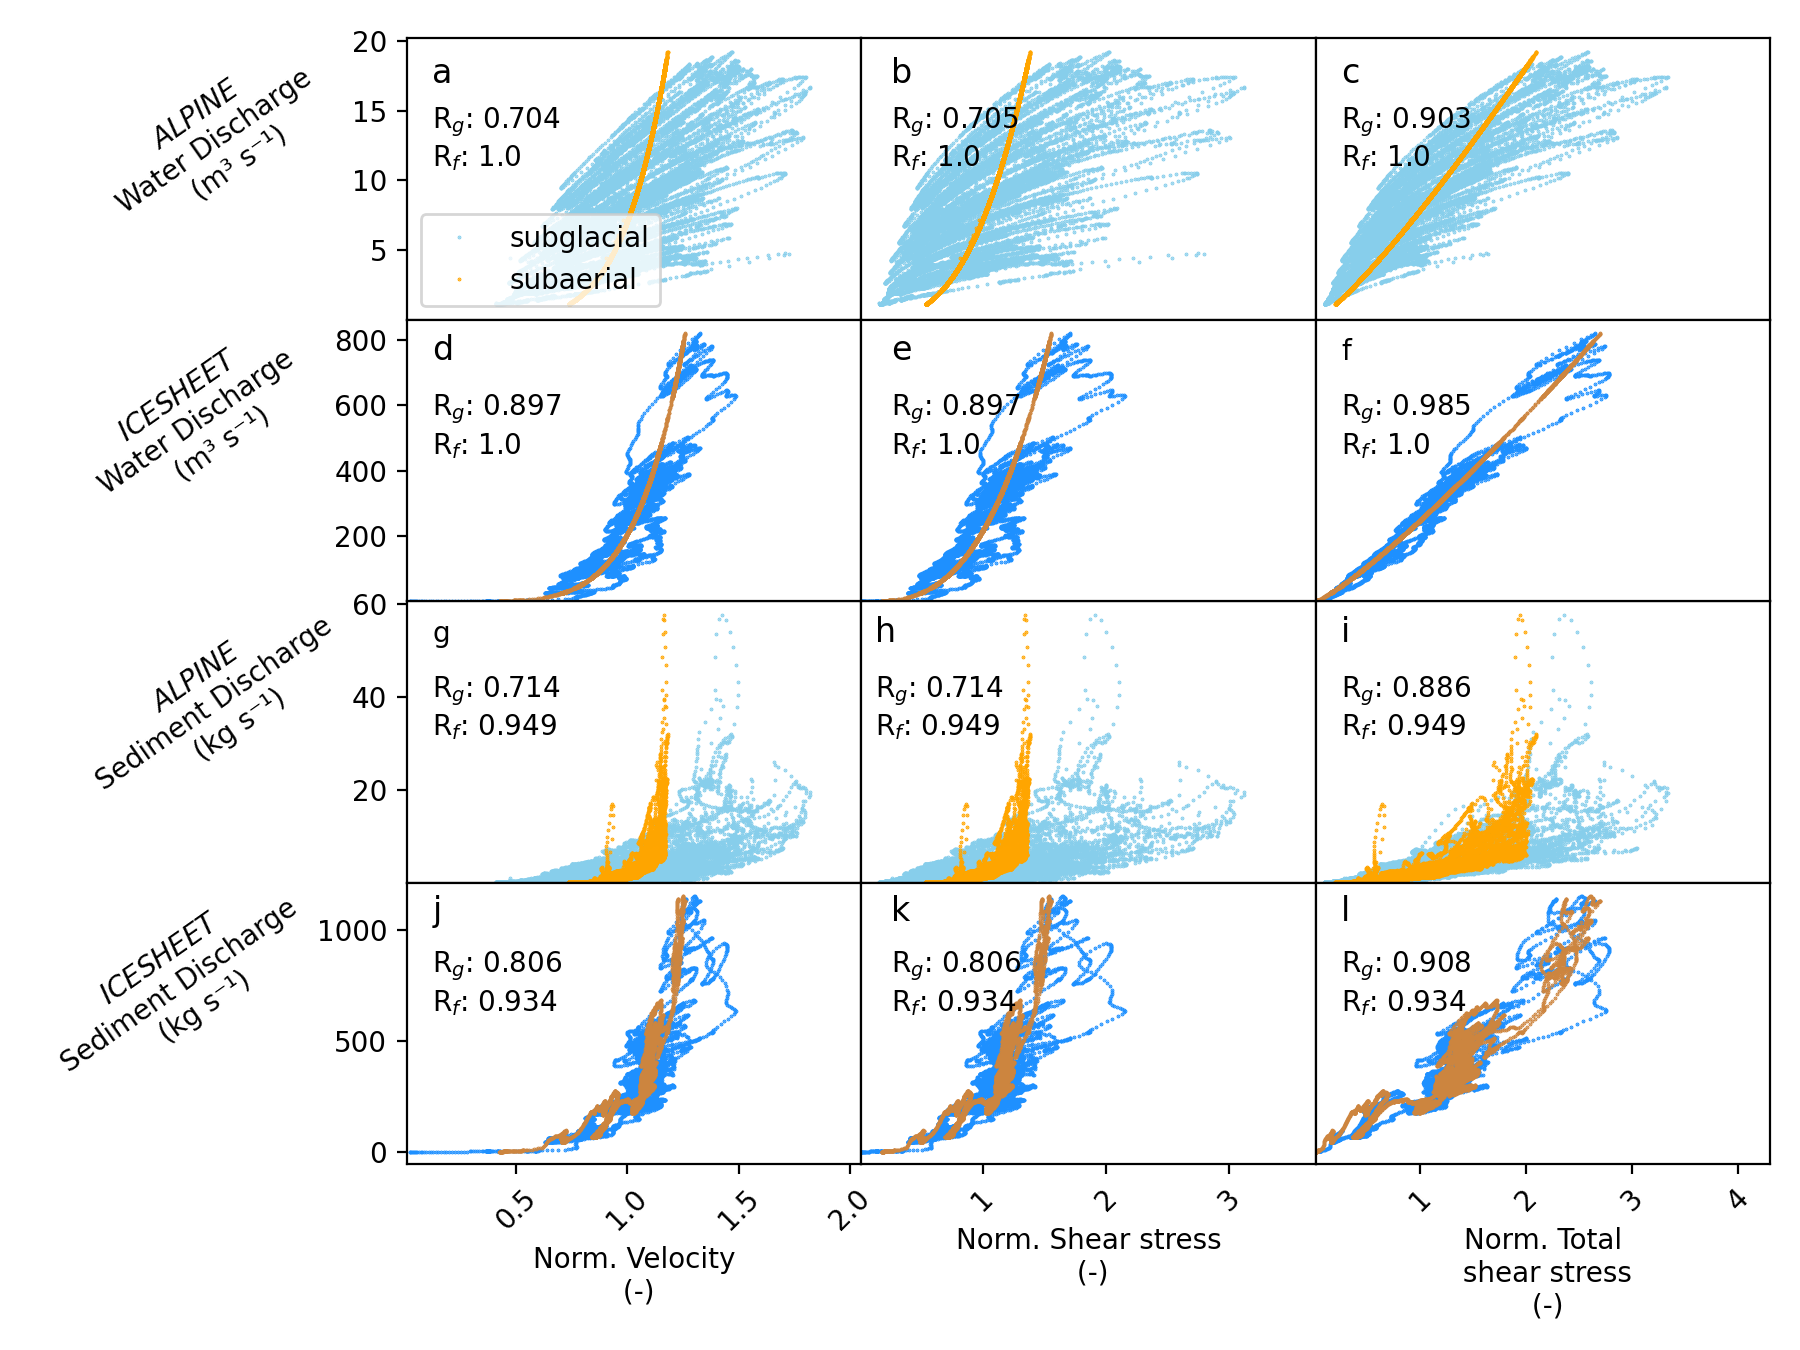
\includegraphics[width=0.7\linewidth]{Fig3_hr.png}
    \caption{As Figure \ref{fig:model_outs}, with $1$ \,\unit{hr} aggregation.}
    \label{fig:model_outs_1hr}
  \end{figure}
\end{center}

\begin{center}
  \begin{figure}[!h]
    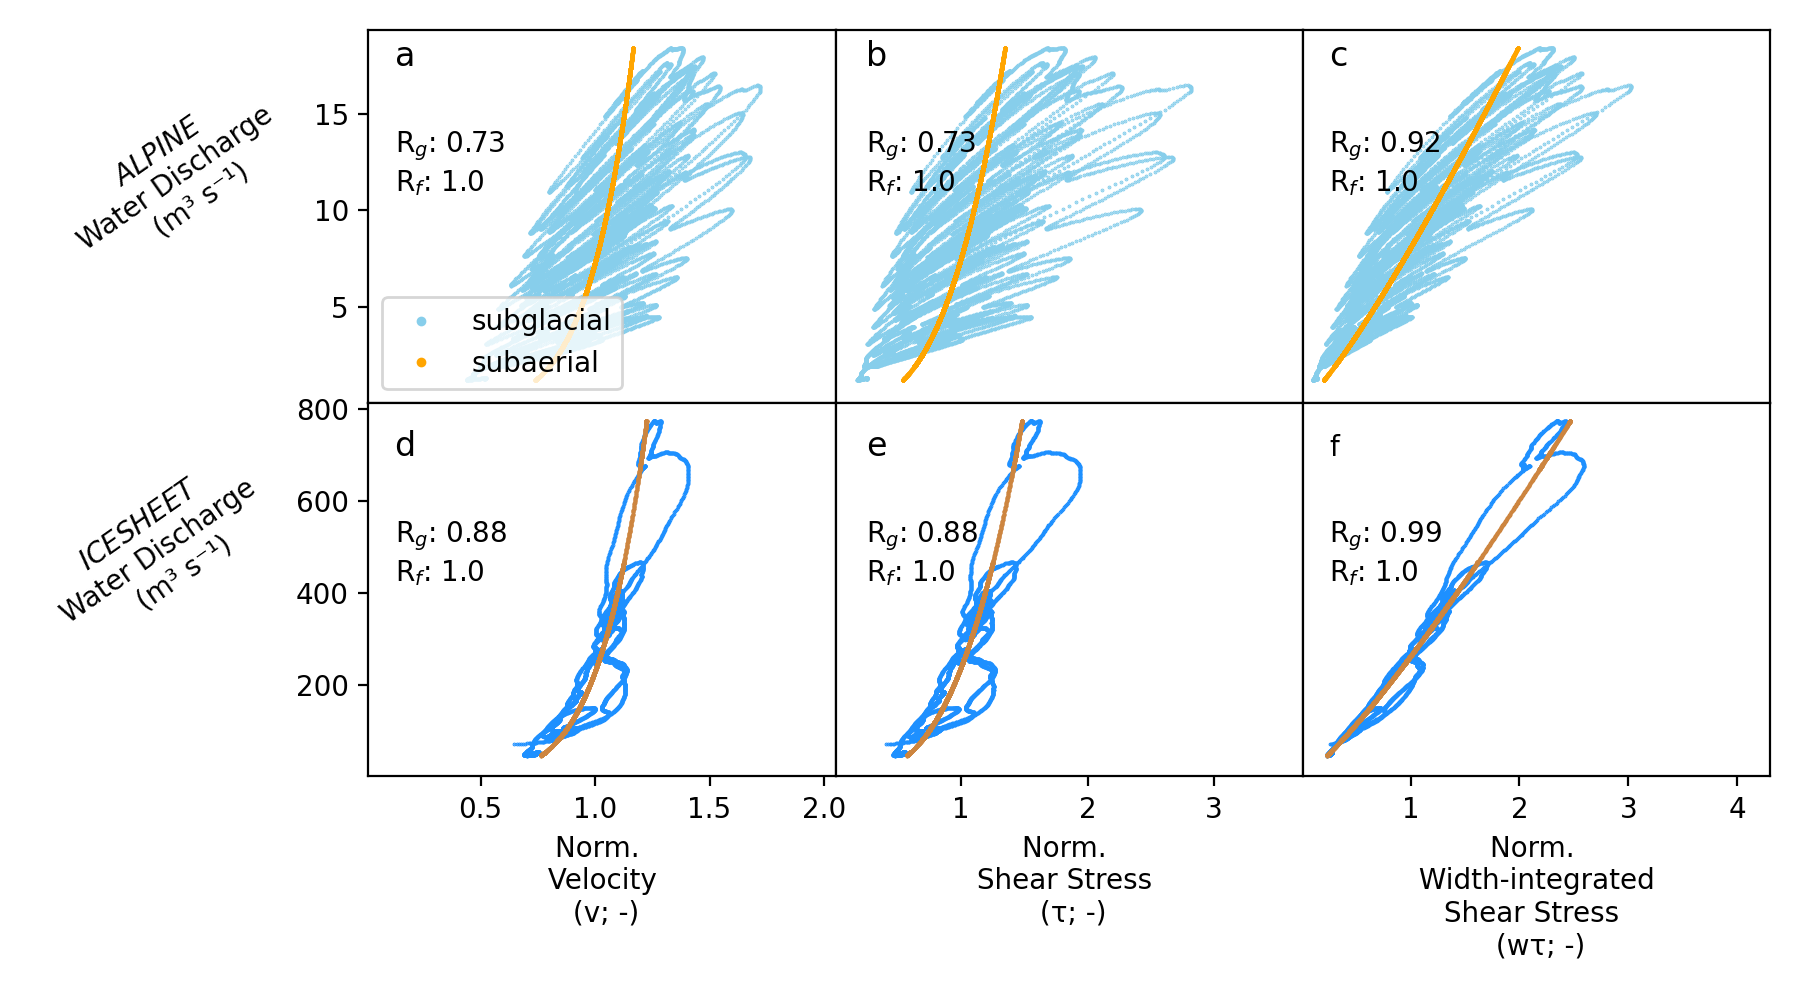
\includegraphics[width=0.7\linewidth]{Fig3_12hr.png}
    \caption{As Figure \ref{fig:model_outs}, with $12$ \,\unit{hr} aggregation.}
    \label{fig:model_outs_12hr}
  \end{figure}
\end{center}


\begin{center}
  \begin{figure}[!h]
    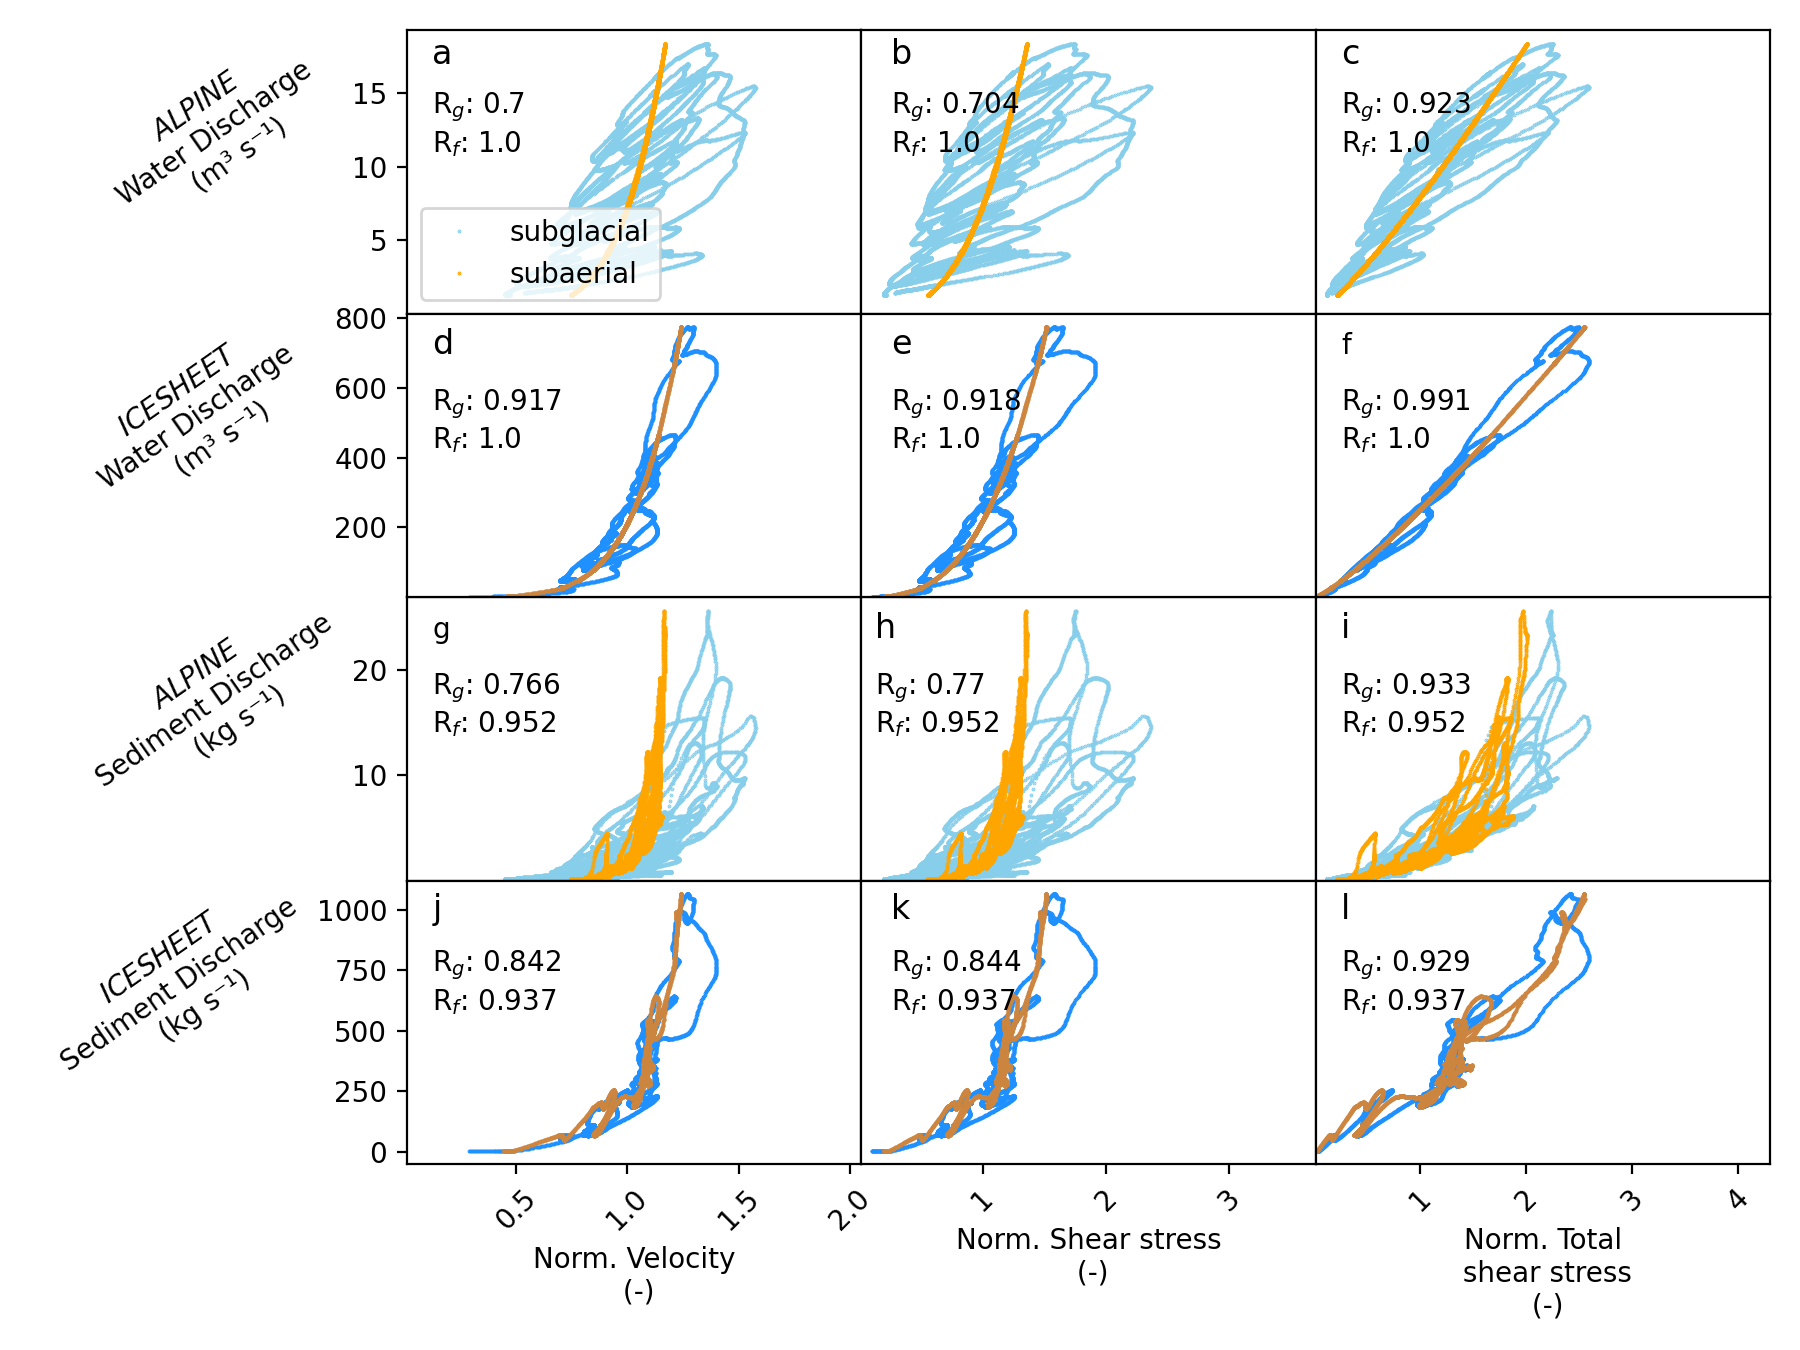
\includegraphics[width=0.7\linewidth]{Fig3_1day.png}
    \caption{As Figure \ref{fig:model_outs}, with $1$ \,\unit{day} aggregation.}
    \label{fig:model_outs_1day}
  \end{figure}
\end{center}


\begin{center}
  \begin{figure}[!h]
    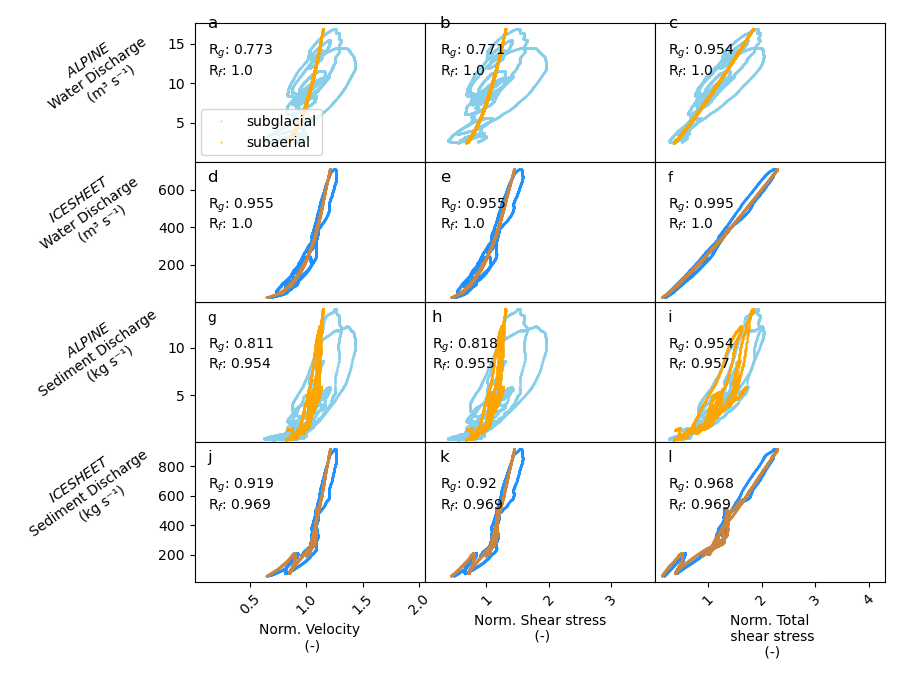
\includegraphics[width=0.7\linewidth]{Fig3_5day.png}
    \caption{As Figure \ref{fig:model_outs}, with $5$ \,\unit{day} aggregation.}
    \label{fig:model_outs_5day}
  \end{figure}
\end{center}

\begin{center}
  \begin{figure}[!h]
    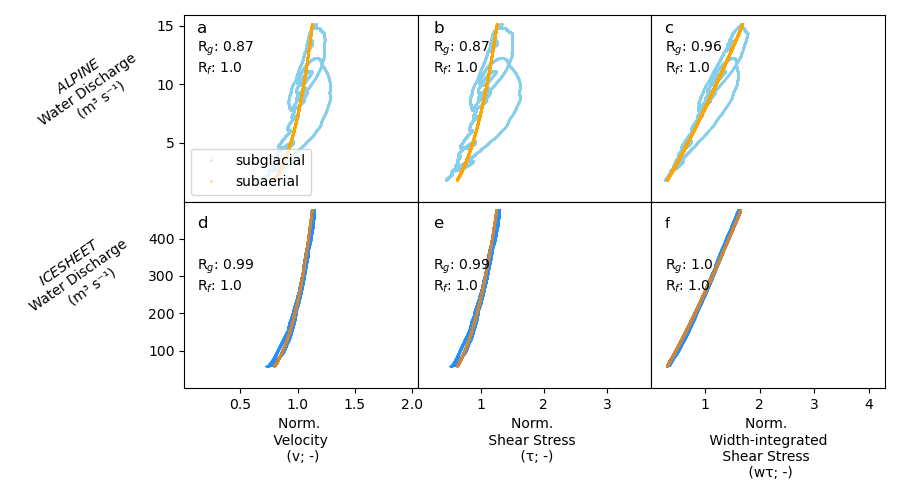
\includegraphics[width=0.7\linewidth]{Fig3_10day.png}
    \caption{As Figure \ref{fig:model_outs}, with $10$ \,\unit{day} aggregation.}
    \label{fig:model_outs_10day}
  \end{figure}
\end{center}

\begin{center}
  \begin{figure}[!h]
    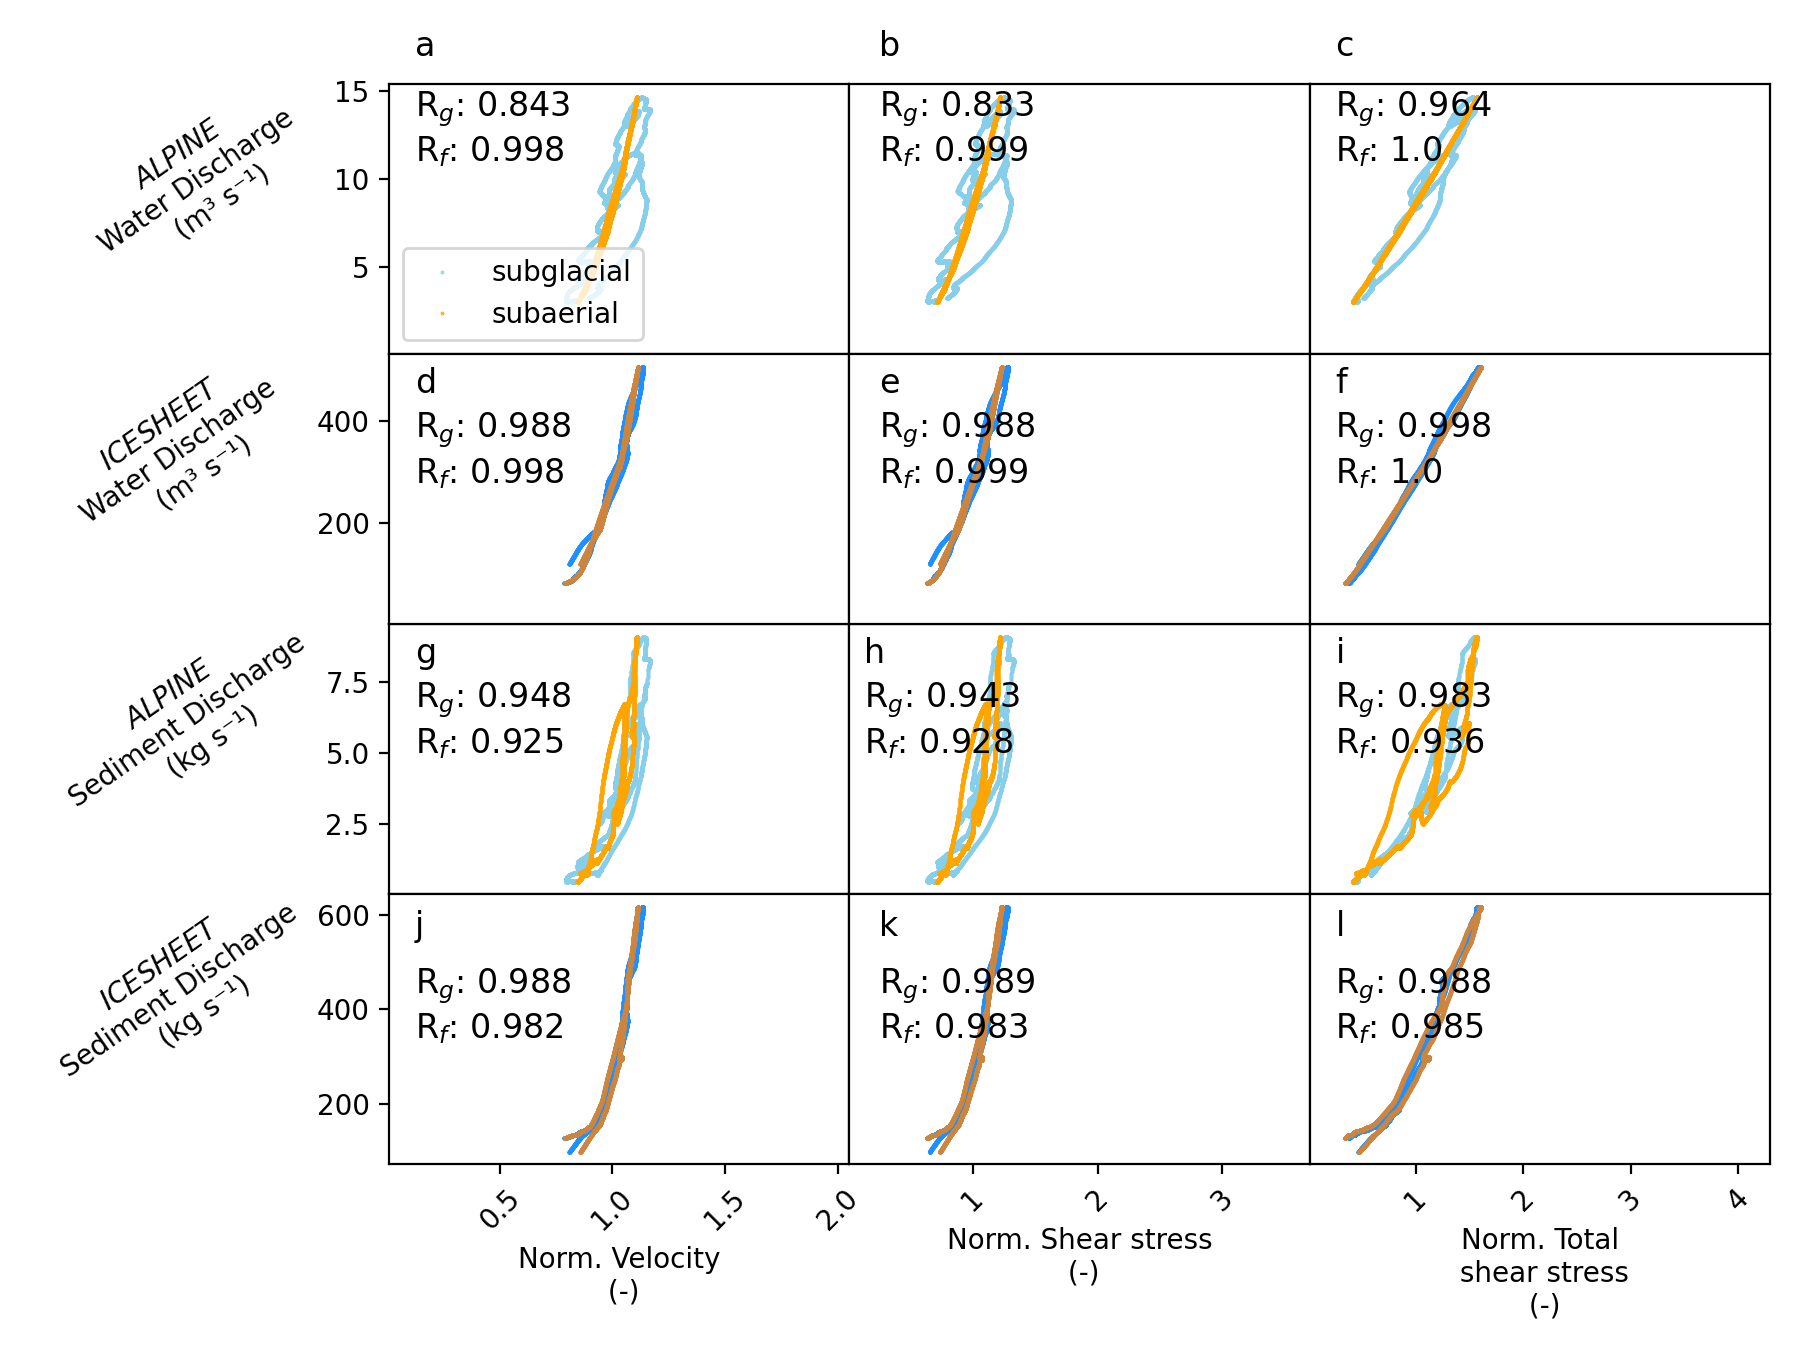
\includegraphics[width=0.7\linewidth]{Fig3_15day.png}
    \caption{As Figure \ref{fig:model_outs}, with $15$ \,\unit{day} aggregation.}
    \label{fig:model_outs_15day}
  \end{figure}
\end{center}
\FloatBarrier



\newpage
\section{Formulas for sediment transport in different drainage regimes}
\label{sect:scaling}

\mauro{Notation: either use $H$ and $W$ for the river, or otherwise, somehow free $h$. Below I use $H$ and $W$ for now.}

Here we look at three kind of drainage regimes, namely, rivers, steady-state R-channels, and pipe-flow (i.e. R-channels which do not have time to adjust their size to discharge conditions).  We calculate how in these regimes sediment flux scales with respect to a given discharge for three different transport formulas: MPM \cite{meyer1948}, EH \cite{engelund1967}, and Bagnold \cite{Bagnold1980}; additionally we state the width integrated shear stress used as proxy for sediment transport throughout the manuscript.

A few basic hydraulic relations are used in the following.  The Darcy-Weisbach equation can be stated as
\begin{equation}
  \label{eq:DW}
  \Psi \propto f\frac{Q^2}{D_h S^2},
\end{equation}
with $\Psi$ the head gradient and friction factor $f$.  The shear stress and stream power are, respectively,
\begin{equation}
    \label{eq:tau-omega}
  \tau \propto f v^2 = f \left(\frac{Q}{S}\right)^2, \quad  \Omega \propto \Psi Q.
\end{equation}
%
Sediment discharge is given by the MPM, EH and Bagnold formulations as, respectively,
\begin{equation}
  Q_s \propto W\, \tau^{3/2}, \quad Q_s \propto W\, \tau^{5/2}, \quad Q_s \propto W \left(\frac{\Omega}{W}\right)^{3/2} H^{-2/3}
\end{equation}
for conditions well above the transport onset threshold.

The river is assumed to have a width $W$ much greater than its depth $H$, such that $D_h\approx 4H$, and to have a constant head gradient ($\Psi$) given by the topography.  Further, we assume that its width can be approximated by a relation $W \propto Q^\alpha$ with $\alpha\in [0,1]$; typically $\alpha \approx 1/2$ (a so-called regime channel), $\alpha=0$ or $\alpha=1$ correspond a river of constant width (a slot canyon) or depth (no natural equivalent), respectively, i.e. the two end members.
%
For a steady state R-channel, we assume that it has a constant $\Psi$ (approximated by the gradient of the Shreve \citeyear{shreve1972} potential) and that $S$ adjusts such that it is in steady state corresponding to $\Psi$ and $Q$.  %Conversely, pipe flow has $S$ fixed and $\Psi$ adjusts to satisfy the given $Q$.
%
For pipe flow, which occurs when a R-channel is subjected to rapid discharge variations such that it cannot adjust its size significantly,  we assume that the cross-sectional area $S$ is fixed and that $\Psi$ adjusts to meet the specified $Q$.  For both R-channel and pipe flow, we assume that $D_h \propto S^{1/2}$.

With these assumptions the Darcy-Weisbach equation~\eqref{eq:DW} can be solved for the not-fixed quantity: $H$ for a river, $S$ for a R-channel, and $\Psi$ for pipe-flow.  Then, using equations~\eqref{eq:tau-omega}, the shear stress and stream power can be calculated.  These results are summarised in Table~\ref{tab:eqs1}.
Now width integrated shear stress and sediment transport can be calculated for all regimes and for all transport formulas.  The results of the 12 combinations are presented in Table~\ref{tab:Qs} and also in Table~\ref{tab:Qs2} where the fractions in the exponents are approximately given by decimal numbers for ease of comparison.

Table~\ref{tab:Qs2} shows that the proxy $W\tau$ as well as the MPM, EH and Bagnold sediment transport formulas give roughly a similar scaling of $Q_s$ on $\Psi$ or $S$ and on $Q$.  Remarkably, the Bagnold formula has a negative exponent for $f$ in all but the pipe-flow regime, which seems rather unexpected.  The total transport formula EH gives a slightly stronger dependence on all variables as should be expected due to to the larger exponent on $\tau$ of 2.5 versus 1.5 for the others.  Albeit, for pipe-flow Bagnold is close to EH. Conversely, the proxy used within this publication scales only as $Q^2$ for pipe-flow, whereas the others scale at least with $Q^3$.  The exponent for the width scaling $\alpha$ only impacts the EH relation in any meaningful way; but for the value of $\alpha$ around 0.5, as is suitable for a braided proglacial stream and indeed most rivers, the exponent on $Q$ is only slightly above what the other relations give.

The sediment discharge in the steady state R-channel scales very similarly to the river case for all relations and virtually identically for the $\alpha=0.5$ case.  However, note that the head gradients $\Psi$ are likely higher for comparable $Q$ in a ice-sheet marginal or alpine glacier setting than in a river setting, as is well described in \citeA{alley1997}, and thus transport rates may still be much higher in a steady state R-channel.

Furthermore, R-channels will rarely operate in steady state as variations in discharge, in particular on the diurnal timescale or the timescale of severe rain or melting events, are too fast for such a channel to reach a steady state.  In such cases they operate more like a pipe of fixed cross-section.  Table~\ref{tab:Qs2} shows that in such a situation, the sediment transport scales much more severely with discharge, with the exponent of $Q$ being likely between 3 and 5, compared to other two regimes when that exponent is at most 1.3.  Thus fluctuations of discharge on short timescales (on the order of a day) have the potential to cause very high sediment transport conditions.

\begin{table}
  \caption{Relations for hydraulic variables for the three drainage regimes: river, R-channel and pipe-flow.  Darcy-Weisbach equation is abbreviated with ``D-W'', and stream power with ``Stream p.''. }
  \label{tab:eqs1}
  \small
\begin{tabular}{llllll}
Regime & Fixed & Determined via D-W & Additional relations & Shear stress & Stream p.\\
 &  &  &  & \(\tau \propto\) & \(\Omega \propto\)\\
\hline
River & \(\Psi\) & \(H \propto f^{1/3}\, Q^{2/3-2\alpha/3} \, \Psi^{-1/3}\) & \(W\,\propto Q^\alpha\), \(S=WH\), \(D_h=H\) & \(f^{1/3} Q^{2/3-2\alpha/3}  \Psi^{2/3}\) & \(Q \Psi\)\\
R-ch. & \(\Psi\) & \(S\, \propto f^{2/5}\, Q^{4/5} \, \Psi^{-2/5}\) & \(D_h\propto W \propto H \propto S^{1/2}\) & \(f^{1/5} Q^{2/5} \, \Psi^{4/5}\) & \(Q \Psi\)\\
Pipe & \(S\) & \(\Psi \propto f \, Q^2\, S^{-5/2}\) & \(D_h\propto W \propto H \propto S^{1/2}\) & \(f Q^2 S^{-2}\) & \(f Q^3 S^{-5/2}\)\\
\end{tabular}
\end{table}


\begin{table}
  \caption{Sediment transport proxy ($W\tau$) and rates for the three considered different transport formulas: MPM \cite{meyer1948}, EH \cite{engelund1967}, and Bagnold \cite{Bagnold1980}.
    }
  \label{tab:Qs}
\begin{tabular}{lllll}
 & Width*\(\tau\) & MPM & EH & Bagnold\\
 & \(W\, \tau\) & \(Q_s \propto W\, \tau^{3/2}\) & \(Q_s \propto W\, \tau^{5/2}\) & \(Q_s \propto W^{-1/2}\, \Omega^{3/2} H^{-2/3}\)\\
\hline
River & \(f^{1/3}\, Q^{2/3+\alpha/3}\,  \Psi^{2/3}\) & \(f^{1/2}\, Q \, \Psi\) & \(f^{5/6}\, Q^{5/3 - 2\alpha/3} \, \Psi^{5/3}\) & \(f^{-2/9}\, Q^{19/18-\alpha/18} \, \Psi^{31/18}\)\\
R-ch. & \(f^{2/5}\, Q^{4/5} \, \Psi^{3/5}\) & \(f^{1/2}\, Q \, \Psi\) & \(f^{7/10}\, Q^{7/5}\, \Psi^{9/5}\) & \(f^{-7/30}\, Q^{31/30}\, \Psi^{26/15}\)\\
Pipe & \(f \, Q^2 \, S^{-1}\) & \(f^{3/2}\, Q^3 \, S^{-5/2}\) & \(f^{5/2}\, Q^5\, S^{-9/2}\) & \(f^{3/2} \, Q^{9/2} \, S^{-14/3}\)\\
\end{tabular}
\end{table}

\begin{table}
  \caption{As Table~\ref{tab:Qs} but with the fractional exponents stated as rounded decimal numbers.  For the River regime the exponents are for displayed for the likely width-exponent $\alpha=1$, as well as its end members 0 (slot canyon) and 1 (only width increases and not depth).
    }
  \label{tab:Qs2}
\begin{tabular}{lllll}
 & Width*\(\tau\) & MPM & EH & Bagnold\\
 & \(W\, \tau\) & \(Q_s \propto W\, \tau^{3/2}\) & \(Q_s \propto W\, \tau^{5/2}\) & \(Q_s \propto W^{-1/2}\, \Omega^{3/2} H^{-2/3}\)\\
\hline
River (\(\alpha=0\)) & \(f^{0.7}\, Q^{0.7}\,  \Psi^{0.7}\) & \(f^{0.5}\, Q \,\,\,\, \Psi\) & \(f^{0.8}\, Q^{1.7} \, \Psi^{1.7}\) & \(f^{-0.2}\, Q^{1.1} \, \Psi^{1.7}\)\\
River (\(\alpha=0.5\)) & \(f^{0.7}\, Q^{0.8}\,  \Psi^{0.7}\) & \(f^{0.5}\, Q \,\,\,\, \Psi\) & \(f^{0.8}\, Q^{1.3} \, \Psi^{1.7}\) & \(f^{-0.2}\, Q^{1.0} \, \Psi^{1.7}\)\\
River (\(\alpha=1\)) & \(f^{0.7}\, Q^{1.0}\,  \Psi^{0.7}\) & \(f^{0.5}\, Q \,\,\,\, \Psi\) & \(f^{0.8}\, Q^{0.7} \, \Psi^{1.7}\) & \(f^{-0.2}\, Q^{1.0} \, \Psi^{1.7}\)\\[3pt]
R-ch. & \(f^{0.4}\, Q^{0.8} \, \Psi^{0.6}\) & \(f^{0.5}\, Q \,\,\,\, \Psi\) & \(f^{0.7}\, Q^{1.4}\, \Psi^{1.8}\) & \(f^{-0.2}\, Q^{1.0} \, \Psi^{1.7}\)\\
Pipe & \(f \,\quad Q^{2\phantom{.0}} \, S^{-1}\) & \(f^{1.5}\, Q^3 \, S^{-2.5}\) & \(f^{2.5}\, Q^{5\phantom{.0}}\, S^{-4.5}\) & \(f^{1.5} \,\,\,\,\, Q^{4.5} \, S^{-4.7}\)\\
\end{tabular}
\end{table}

\end{document}
